%File: formatting-instructions-latex-2024.tex
%release 2024.0
\documentclass[letterpaper]{article} % DO NOT CHANGE THIS
\usepackage{aaai24}  % DO NOT CHANGE THIS
\usepackage{times}  % DO NOT CHANGE THIS
\usepackage{helvet}  % DO NOT CHANGE THIS
\usepackage{courier}  % DO NOT CHANGE THIS
\usepackage[hyphens]{url}  % DO NOT CHANGE THIS
\usepackage{graphicx} % DO NOT CHANGE THIS
\usepackage{indentfirst}
\usepackage[portuguese]{babel}
\urlstyle{rm} % DO NOT CHANGE THIS
\def\UrlFont{\rm}  % DO NOT CHANGE THIS
\usepackage{natbib}  % DO NOT CHANGE THIS AND DO NOT ADD ANY OPTIONS TO IT
\usepackage{caption} % DO NOT CHANGE THIS AND DO NOT ADD ANY OPTIONS TO IT
\frenchspacing  % DO NOT CHANGE THIS
\setlength{\pdfpagewidth}{8.5in}  % DO NOT CHANGE THIS
\setlength{\pdfpageheight}{11in}  % DO NOT CHANGE THIS
%
% These are recommended to typeset algorithms but not required. See the subsubsection on algorithms. Remove them if you don't have algorithms in your paper.
\usepackage{algorithm}
\usepackage{algorithmic}

%
% These are are recommended to typeset listings but not required. See the subsubsection on listing. Remove this block if you don't have listings in your paper.
\usepackage{newfloat}
\usepackage{listings}
\DeclareCaptionStyle{ruled}{labelfont=normalfont,labelsep=colon,strut=off} % DO NOT CHANGE THIS
\lstset{%
	basicstyle={\footnotesize\ttfamily},% footnotesize acceptable for monospace
	numbers=left,numberstyle=\footnotesize,xleftmargin=2em,% show line numbers, remove this entire line if you don't want the numbers.
	aboveskip=0pt,belowskip=0pt,%
	showstringspaces=false,tabsize=2,breaklines=true}
\floatstyle{ruled}
\newfloat{listing}{tb}{lst}{}
\floatname{listing}{Listing}
%
% Keep the \pdfinfo as shown here. There's no need
% for you to add the /Title and /Author tags.
\pdfinfo{
/TemplateVersion (2024.1)
}

% DISALLOWED PACKAGES
% \usepackage{authblk} -- This package is specifically forbidden
% \usepackage{balance} -- This package is specifically forbidden
% \usepackage{color (if used in text)
% \usepackage{CJK} -- This package is specifically forbidden
% \usepackage{float} -- This package is specifically forbidden
% \usepackage{flushend} -- This package is specifically forbidden
% \usepackage{fontenc} -- This package is specifically forbidden
% \usepackage{fullpage} -- This package is specifically forbidden
% \usepackage{geometry} -- This package is specifically forbidden
% \usepackage{grffile} -- This package is specifically forbidden
% \usepackage{hyperref} -- This package is specifically forbidden
% \usepackage{navigator} -- This package is specifically forbidden
% (or any other package that embeds links such as navigator or hyperref)
% \indentfirst} -- This package is specifically forbidden
% \layout} -- This package is specifically forbidden
% \multicol} -- This package is specifically forbidden
% \nameref} -- This package is specifically forbidden
% \usepackage{savetrees} -- This package is specifically forbidden
% \usepackage{setspace} -- This package is specifically forbidden
% \usepackage{stfloats} -- This package is specifically forbidden
% \usepackage{tabu} -- This package is specifically forbidden
% \usepackage{titlesec} -- This package is specifically forbidden
% \usepackage{tocbibind} -- This package is specifically forbidden
% \usepackage{ulem} -- This package is specifically forbidden
% \usepackage{wrapfig} -- This package is specifically forbidden
% DISALLOWED COMMANDS
% \nocopyright -- Your paper will not be published if you use this command
% \addtolength -- This command may not be used
% \balance -- This command may not be used
% \baselinestretch -- Your paper will not be published if you use this command
% \clearpage -- No page breaks of any kind may be used for the final version of your paper
% \columnsep -- This command may not be used
% \newpage -- No page breaks of any kind may be used for the final version of your paper
% \pagebreak -- No page breaks of any kind may be used for the final version of your paperr
% \pagestyle -- This command may not be used
% \tiny -- This is not an acceptable font size.
% \vspace{- -- No negative value may be used in proximity of a caption, figure, table, section, subsection, subsubsection, or reference
% \vskip{- -- No negative value may be used to alter spacing above or below a caption, figure, table, section, subsection, subsubsection, or reference

\setcounter{secnumdepth}{2} %May be changed to 1 or 2 if section numbers are desired.

% The file aaai24.sty is the style file for AAAI Press
% proceedings, working notes, and technical reports.
%

% Title


\title{Universidade Federal de Minas Gerais \\[10pt]
DCC642 - Introdução à Inteligência Artificial (2025/2) \\
 TP1: Busca no Espaço de Estados}
\author {
    Raphael Henrique Braga Leivas - 2020028101
}


\begin{document}

\maketitle


\section{Introdução}

Neste trabalho, algoritmos de busca são implementados em Python para encontrar o caminho 
de menor custo em um mapa com estrutura de grade. Os algoritmos são comparados em diferentes mapas 
para verificar experimentalmente as diferenças entre eles.

\section{Objetivos}

Os objetivos principais do trabalho são: 

\begin{itemize}
	\item Implementar em Python os algoritmos de busca em largura (BFS),
	busca em profundidade (DFS), busca de custo uniforme (UCS), busca gulosa 
	por melhor escolha (Greedy) e busca A*, com heurísticas euclidiana e de Manhattan;
	\item Comparar os algoritmos em 7 casos de teste com diferentes mapas, comparando 
	não só os caminhos retornados, mas também o número de nós expandidos e o custo do 
	caminho final.
\end{itemize}

\section{Casos de Teste}

Nesta seção são abordados 7 casos de teste para evidenciar as principais 
diferenças entre os algoritmos estudados.


\subsection{BFS não é ótimo}

O BFS não garante otimalidade se os custos forem diferentes, como 
mostra a Figura \ref{fig:BFS_nao_otimo}.

\begin{figure}[htb]
	\centering 
    \caption{Caso em que o BFS não é ótimo. (a) Mapa inicial, (b)
	caminho retornado pelo BFS, (c) caminho ótimo encontrado pelo UCS.}
	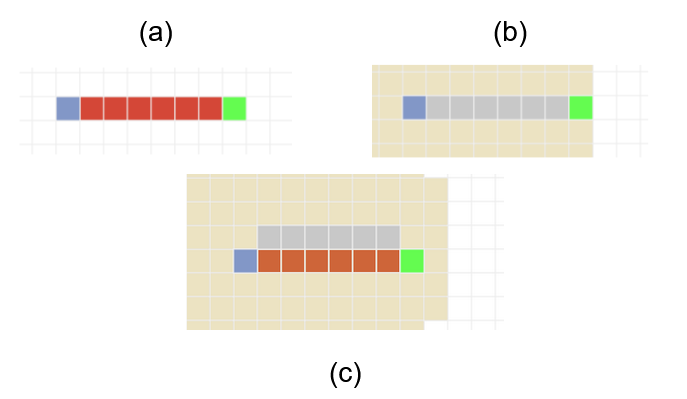
\includegraphics[width=\columnwidth]{images/BFS_nao_otimo.png}
	\label{fig:BFS_nao_otimo}
\end{figure}

Na Figura \ref{fig:BFS_nao_otimo} (a), temos que o caminho direto do início ao alvo 
passa por casas de custo elevado (9), enquanto as demais casas possuem custo unitário.
O BFS, por explorar os nós em camadas, acaba encontrando o caminho (b) que vai diretamente 
até o alvo, passando pelos nós custosos e retornando um caminho de custo total 55.

Contudo, claramente existe um camingo melhor que passa pelos nós de custo unitário.
Assim, usando o UCS é possível encontrar o caminho da Figura \ref{fig:BFS_nao_otimo} (c), 
com custo total 8, que é a solução ótima para o problema.

\subsection{BFS é equivalente à UCS}

BFS e UCS são equivalentes quando todos os custos são iguais \cite{russell2020aima}, como mostra 
a Figura \ref{fig:BFS_UCS_equiv} (a). Todas as arestas do mapa possuem
 custo unitário, de modo que a solução encontrada pelo BFS na Figura \ref{fig:BFS_UCS_equiv} (b) 
 é igual à solução do UCS na Figura \ref{fig:BFS_UCS_equiv} (c). Além disso, note que 
 a maneira em que os nós são explorados é bastante parecida, avançando radialmente 
 a partir do nó inicial.


\begin{figure}[htb]
	\centering 
    \caption{Caso em que o BFS e o UCS são equivalentes. (a) Mapa inicial, (b)
	caminho retornado pelo BFS, (c) caminho retornado pelo UCS.}
	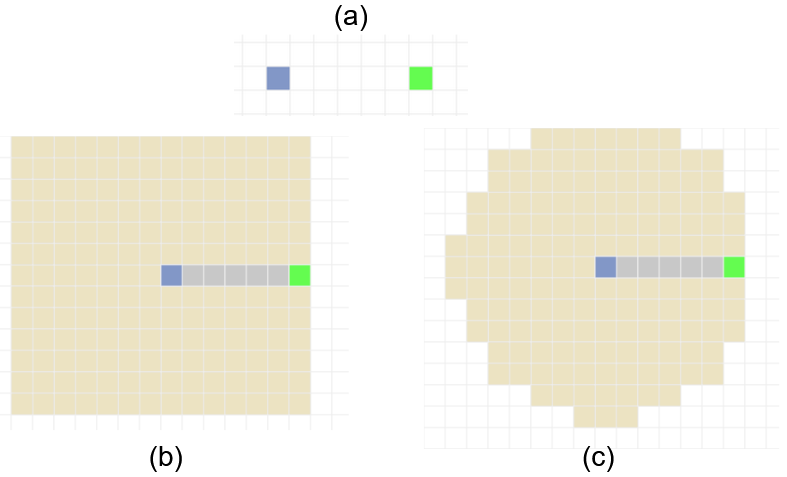
\includegraphics[width=\columnwidth]{images/BFS_UCS_equiv.png}
	\label{fig:BFS_UCS_equiv}
\end{figure}


\subsection{DFS retorna a solução ótima}

O DFS em geral não é ótimo uma vez que ele retorna o primeiro caminho encontrado
e não necessariamente o de menor custo. Contudo, em alguns casos o DFS pode
retornar a solução ótima, como mostra a Figura \ref{fig:DFS_otimo} (a), em que 
todos os custos são iguais e todas as soluções possíveis possuem a mesma 
profundidade.

\begin{figure}[htb]
	\centering 
    \caption{Caso em que o DFS garante otimalidade. (a) Mapa inicial, (b)
	caminho retornado pelo DFS.}
	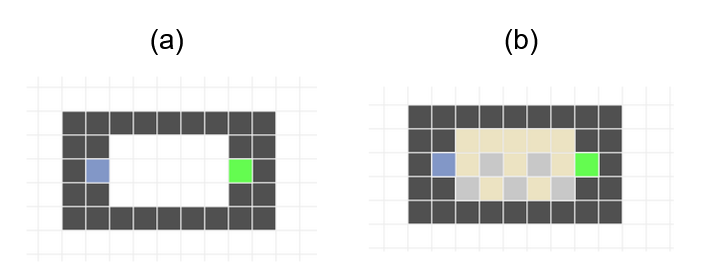
\includegraphics[width=\columnwidth]{images/DFS_otimo.png}
	\label{fig:DFS_otimo}
\end{figure}

Note que esse caso é bastante específico e não é possível garantir que o DFS
sempre retorne a solução ótima. 

\subsection{Greedy é ótimo}\label{sec:greedy_otimo}

A busca gulosa pela melhor escolha (Greedy) é ótima se todos os custos 
forem iguais. A Figura \ref{fig:greedy_otimo} (a) mostra um mapa em que
todos os custos são unitários, de modo que o Greedy retorna o caminho
da Figura \ref{fig:greedy_otimo} (b), que é ótimo.

\begin{figure}[htb]
	\centering 
    \caption{Caso em que o Greedy garante otimalidade (heurística euclidiana). (a) Mapa inicial, (b)
	caminho retornado pelo Greedy.}
	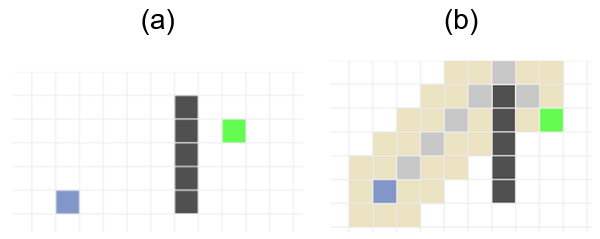
\includegraphics[width=\columnwidth]{images/greedy_otimo.png}
	\label{fig:greedy_otimo}
\end{figure}

\subsection{Greedy não é ótimo}

No entanto, ao contrário no visto na Seção \ref{sec:greedy_otimo},  
se os custos forem diferentes, o Greedy pode não ser ótimo, como 
mostra a Figura \ref{fig:greedy_nao_otimo} (a). De forma similar ao visto com o BFS 
na Figura \ref{fig:BFS_nao_otimo}, o Greedy acaba escolhendo o caminho que vai direto para 
o alvo, passando por nós de custo elevado (9) e retornando um caminho de custo total 43.48, sendo que 
o UCS na Figura \ref{fig:greedy_nao_otimo} (c) encontra o caminho ótimo, com custo total 12.

\begin{figure}[htb]
	\centering 
    \caption{Caso em que o Greedy não garante otimalidade (heurística euclidiana). (a) Mapa inicial, (b)
	caminho retornado pelo Greedy e (c) caminho ótimo retornado pelo UCS.}
	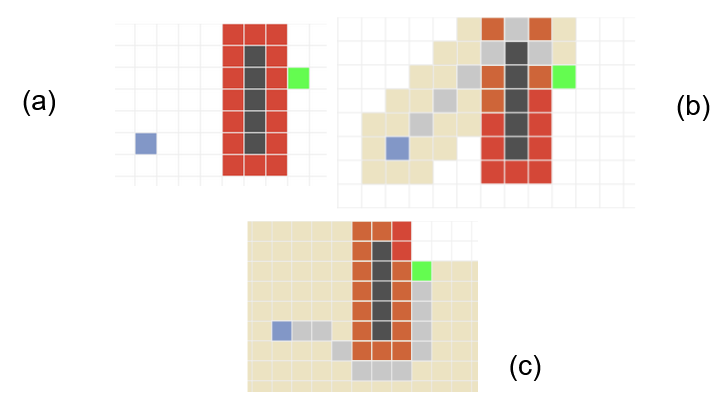
\includegraphics[width=\columnwidth]{images/greedy_nao_otimo.png}
	\label{fig:greedy_nao_otimo}
\end{figure}


\subsection{A* é melhor que UCS}

Como o A* utiliza uma heurística para guiar a busca, ele pode ser mais eficiente
que o UCS, como mostra a Figura \ref{fig:astar_melhor_ucs} (a). Nesse caso, o A*
retorna o caminho da Figura \ref{fig:astar_melhor_ucs} (b) expandindo 910 nós enquato o 
 UCS retorna o caminho da Figura \ref{fig:astar_melhor_ucs} (c) expandindo 1146 nós.
\begin{figure}[htb]
	\centering 
    \caption{Caso em que o A* pode ser melhor do que o UCS (heurística euclidiana). (a) Mapa inicial, 
	(b) caminho retornado pelo A*, e (c)
	caminho retornado pelo UCS.}
	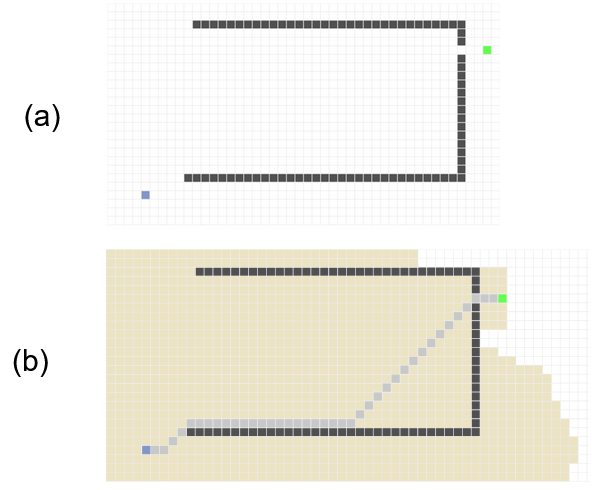
\includegraphics[width=\columnwidth]{images/astar_melhor_ucs_p1.png}
	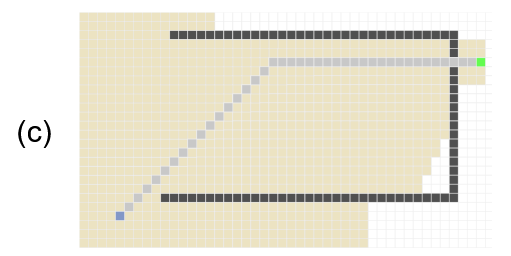
\includegraphics[width=\columnwidth]{images/astar_melhor_ucs_p2.png}
	\label{fig:astar_melhor_ucs}
\end{figure}

Isso ocorre uma vez que a heuirística usada pelo A* direciona a busca, expandindo menos nós durante o processo.
Note que ambos ainda encontram a mesma solução ótima, com custo total 47.04 e tamanho 41.

\subsection{A* é equivalente à UCS}

O A* se torna equivalente ao UCS quando a parcela da heurística tem pouco 
impacto quando somada ao custo do caminho. Assim, se um mapa tiver custos elevados 
em todos os nós, a heurística acaba não influenciando tanto a busca, como mostra a
Figura \ref{fig:astar_equiv_ucs} (a). Nesse caso, o A* retorna o caminho da Figura 
\ref{fig:astar_equiv_ucs} (b) expandindo 114 nós, enquanto o UCS retorna o caminho da 
Figura \ref{fig:astar_equiv_ucs} (c) expandindo 117 nós, praticamente a mesma quantidade.

\begin{figure}[htb]
	\centering 
    \caption{Caso em que o A* pode ser melhor do que o UCS (heurística euclidiana). (a) Mapa inicial, 
	(b) caminho retornado pelo A*, e (c)
	caminho retornado pelo UCS.}
	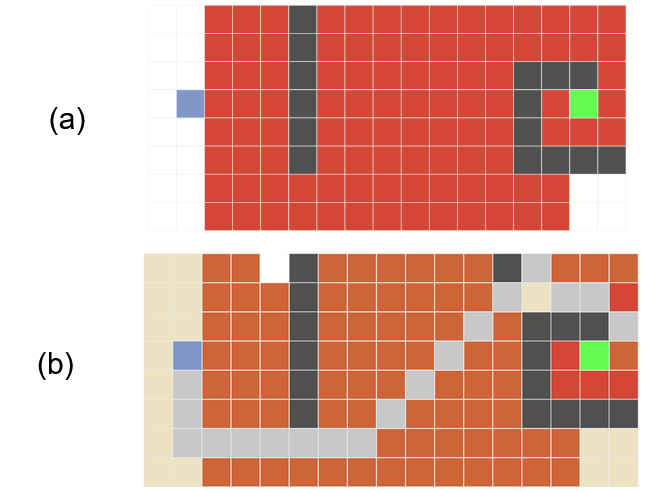
\includegraphics[width=\columnwidth]{images/astar_equiv_ucs_p1.png}
	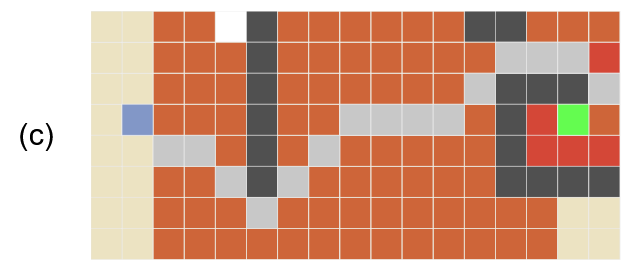
\includegraphics[width=\columnwidth]{images/astar_equiv_ucs_p2.png}
	\label{fig:astar_equiv_ucs}
\end{figure}


\section{Conclusão}

Tendo em vista os objetivos propostos, foi possível implementar os algoritmos de busca
em Python e compará-los em diferentes mapas. Por meio dos casos de teste, foi possível
verificar as diferenças entre os algoritmos, tanto em termos de qualidade das soluções quanto
nos casos em que eles não garantem otimalidade.


\bibliography{aaai24}

\end{document}
